Occupancies close to the beam create many of the key challenges in the HPS experiment
and determine the limits of sensitivity a low A$^\prime$ masses.
These occupancies are dominated by electrons scattered to large angles 
in the converter. Because HPS is sensitive to scattering angles very far out 
on the tail, beyond angles important in other experiments, care must be taken
to ensure our simulations are correct in this regime.  In particular,
Geant4 overestimates the multiple coulomb scattering rate by a factor of two  
at large angles as explained in detail in the appendix (see Fig.~\ref{appendix:2}).
One of the main goals of the test run in 2012 was to evaluate the description of the tails of the multiple coulomb scattering in order 
to gain further confidence in our expected detector occupancy. As will be shown below, data from the 
test run can be used to confirm our model of multiple coulomb scattering despite the fact that 
all data was taken with a photon beam.

Figure~\ref{fig:schematic_testrun_vs_erun} gives a schematic view of the main differences 
between the photon and electron beam setup. 
\begin{figure*}[]
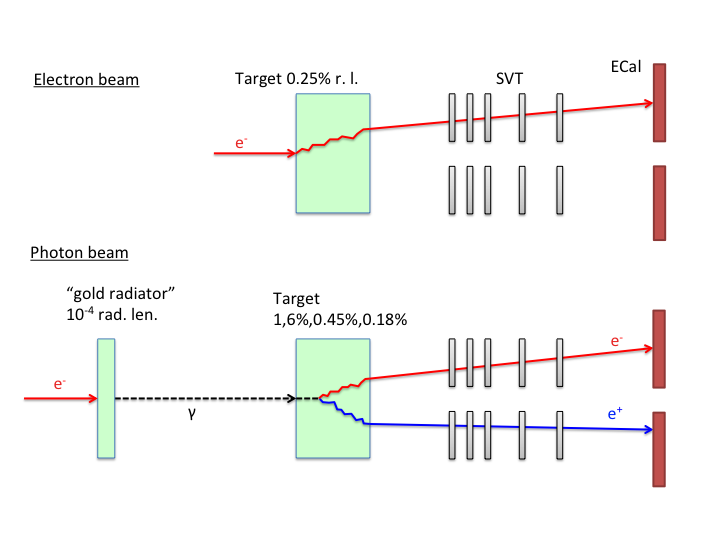
\includegraphics[ scale=0.5]{test2012/angular_measurement/pictures/photon_vs_electron_beam_schematic.png}
\caption{\small{Schematic comparison of the the setup in the test run photon beam compared to the HPS electron beam.}}\label{fig:schematic_testrun_vs_erun}
\end{figure*}
In particular, the angular distribution of the pair produced electron and positions emerging 
from the converter has comparable contributions from {\it i)} the pair production angle
and {\it ii)} the multiple coulomb scattering of the electron and position in the converter after production, see  Fig.~\ref{fig:schematic_pair_prod}.
\begin{figure*}[]
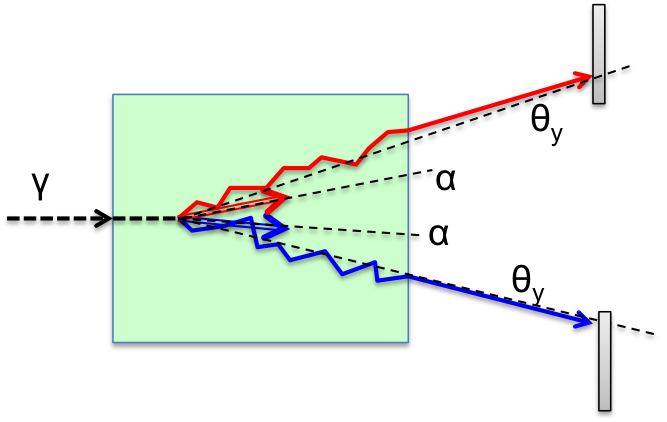
\includegraphics[ scale=0.7]{test2012/angular_measurement/pictures/pair_prod_schematics.png}
\caption{\small{Schematic description of the relevant angles for pair production in the 
test run.}}\label{fig:schematic_pair_prod}
\end{figure*}
%The contribution from the two firsboth sources to the final angular distribution are comparable. 
%FigureX 
%shows the expected distribution of the vertical angle $\theta_y$ for the $e^+e^-$ pair  coming 
%out of the converter compared to the pair production angle. {\color{red} Need this figure from Takashi.} 


%{\bf Sample Composition}\newline

The measured angular distribution in the ECal for the three converter thicknesses are shown in 
Fig.~\ref{fig:ang_distr_data} (left).  
\begin{figure*}[]
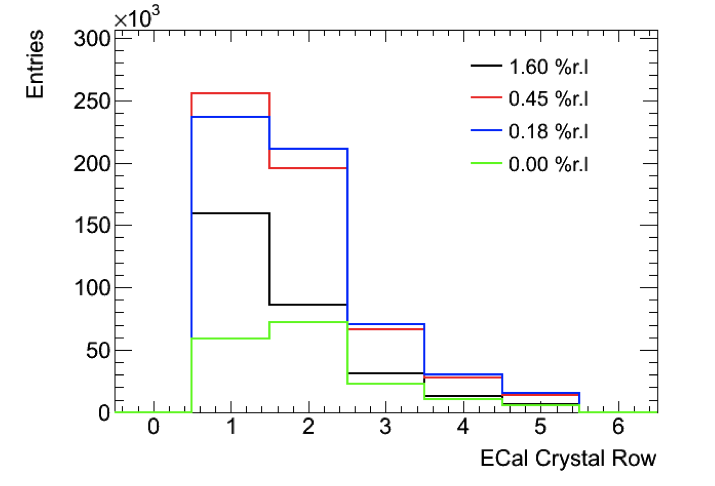
\includegraphics[ scale=0.65]{test2012/angular_measurement/pictures/rate_ecalrow_raw.png}
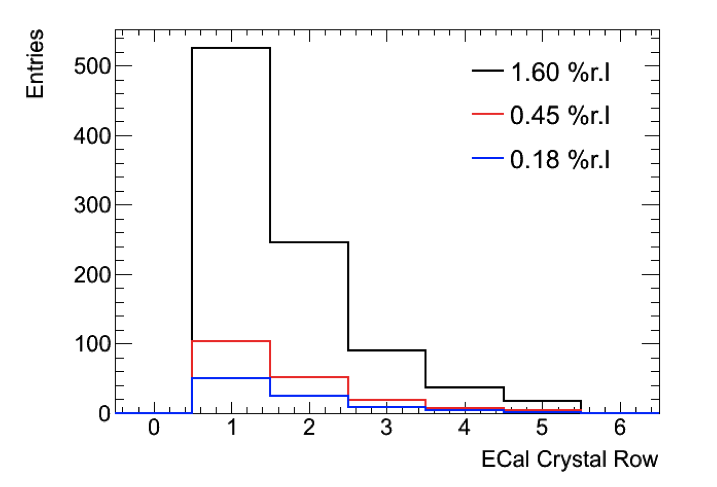
\includegraphics[ scale=0.65]{test2012/angular_measurement/pictures/rate_ecalrow_norm_subtr.png}
\caption{\small{Measured raw vertical angular distributions before (left) and after (right) 
normalization and background subtraction.}}
\label{fig:ang_distr_data}
\end{figure*}
The photon beam line during the test run produced a relatively large fraction of pairs 
originating upstream of the converter. This contribution was measured during data taking 
with "empty" converter runs i.e. removing the converter but with all other conditions 
the same. The upstream background measured in the "empty" converter runs was subtracted 
from the other runs, properly normalized using the measured integrated currents detailed in 
Tab.~\ref{tab:currents}.
\begin{table}
\centering
\begin{tabular}{|c|c|c|}
\hline
%Run & converter thickness [\%r.l.] &   start time[s]      & end time [s] & Duration [s] &       integrated beam current (nC)    \\                thickness (%r.l.)       Rate(Hz)     Recorded(Hz)  Magnet Polarity
Converter thickness & Duration &  $e^-$ on converter \\
 (\%r.l.) & (s) & (nC)    \\   
\hline
%\hline
1.6   & 911 &     24385.9     \\
%\hline
0.18   & 2640 &    193508.9  \\
%\hline
0.45  & 2149 &       140709.9  \\
%\hline
0    & 1279  &   88079.6  \\
%1349    1337323714      1337324625      51344.0926551819        54879.7343788147        1.6                     1262.120     1174.728      -1
%1351    1337324962      1337325268      24385.9185791016        26928.0426635742        1.6                     1933.479     1696.808      -1
%1353    1337325717      1337328357      193508.881838322        204325.132622242        0.18                    436.895      425.659       -1
%1354    1337328521      1337330670      140709.898532331        148839.141475141        0.45                    596.055      570.870       -1
%1358    1337331152      1337332431      88079.5567516331        92523.9428218845        0                       309.785      304.253       -1
%1359    1337332615      1337334014      91653.0026320741        91761.4541434497        0                       318.640      311.540       1
%1360    1337334136      1337336898      198670.590789914        209883.979889035        0.18                    451.067      446.510       1
%1362    1337337264      1337338713      105642.70688653         110298.553449392        1.6                     1864.090     1659.675      1
%1363    1337340178      1337340456      8556.8459701538         8556.8459701538         1.6                     1864.090     1659.675      1
\hline
\end{tabular}
\caption{{\small Measured integrated currents for the runs used to measure the angular distributions.}}
\label{tab:currents}
\end{table}
The background fraction for the there converter thicknesses was 16\%, 52\% and 71\% 
for converter thicknesses of 1.6\%, 0.45\% and 0.18\%, respectively. The background fraction was also 
cross-checked by pointing back tracks reconstructed in the SVT to identify the fraction of tracks not emanating from the converter. This can be seen in Fig.~\ref{fig:extrapol_converter} (bottom) where small 
satellite peaks at $\pm 10$~mm can be identified as tracks fmor the upstream background. The angular distribution, after normalization and subtracting the upstream background, are shown in 
Fig.~\ref{fig:ang_distr_data} (right).  We also checked that the contribution from photons to our triggered 
sample was less than 2\% (without angular selections which would further reduce the contribution).
%. To make sure that our distributions are dominated by $e^+e^-$ pair Since we are primarily interested in measuring the angular 
%distributions for the $e^+e^-$ pair we checked that the contribution from photons in our triggered sample are negligible. Table~\ref{tab:sample_composition} shows the sample composition. The fraction of photons that would deposit energy to reach threshold in the ECal crystals are much less than 2\% without any angular selection which will further reduce the fraction of photons. 
%\begin{table}[]
%\centering
%\begin{tabular}{c|c|c|c}
%Type & Nominal & $E>0.2$~GeV & $E>0.5$~GeV \\
%\hline
%electron & 7150 & 4938 & 3186 \\
%positron & 6019 & 4568 & 2874 \\
%$e^+e^-$ & 13169 & 9506 & 6060 \\
%photon & 2984 & 640 & 151 \\
%\hline
%\end{tabular}
%\caption{Sample composition for the photon test run.}
%\label{tab:sample_composition}
%\end{table}
%Figure~\ref{fig:extrapol_converter} (bottom) shows the vertical position of 
%reconstructed tracks in the SVT during data taking with a converter thickness of 
%1.6\% radiation length. Note the small satellite peaks visible at about $\pm 10$~mm which 
%can be identified as the upstream background when studying the same distribution from the 
%run without any converter. 
%\begin{figure*}[t]
%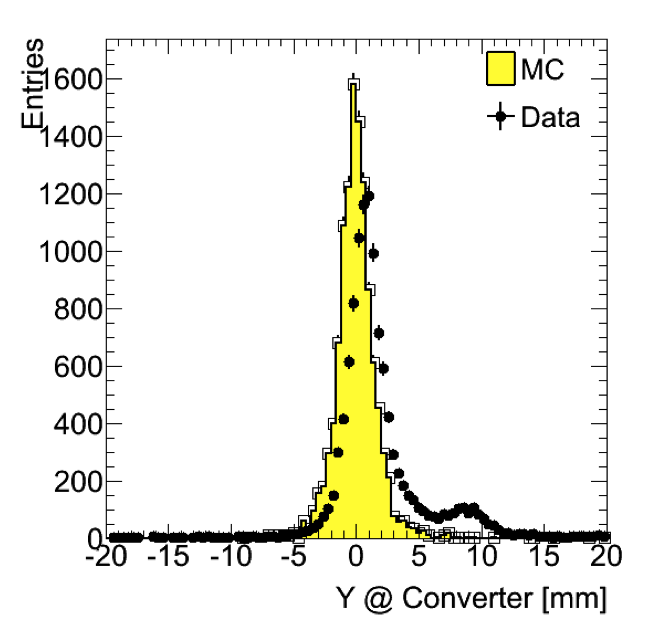
\includegraphics[ scale=0.6]{test2012/angular_measurement/pictures/tracks_at_converter_Y_top.png}
%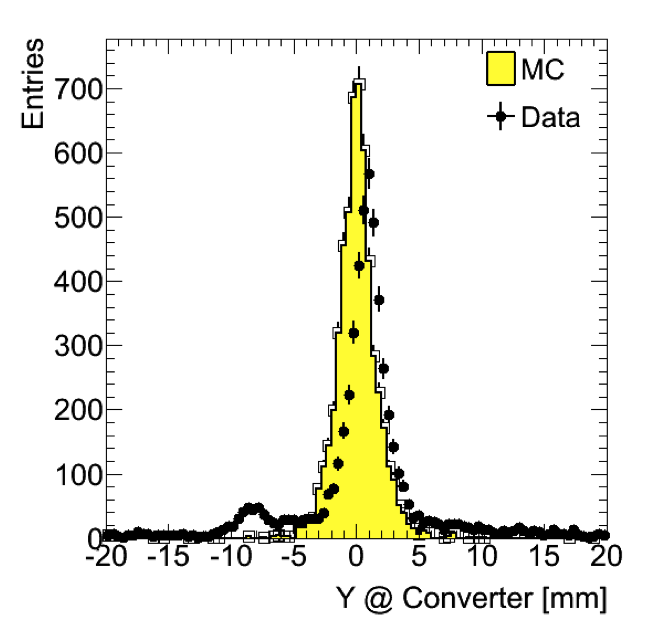
\includegraphics[ scale=0.6]{test2012/angular_measurement/pictures/tracks_at_converter_Y_bottom.png}
%\caption{\small{Vertical position of extrapolated tracks from the SVT to the converter position.} {\color{red}Need update.}}\label{fig:tracks_at_converter}
%\end{figure*}


These measured angular distributions are then compared to simulation to validate the modeling of the 
multiple coulomb scattering. As described in more detail in the appendix, EGS5 is used to generate 
the electromagnetic interactions in the converter while GEANT4 is used to simulate the particles after the converter.  Figure~\ref{fig:ang_distr_dataMC} shows the angular distribution comparing data and 
EGS5 normalized to 1~s of beam at 90~nA beam current. 
\begin{figure*}[t]
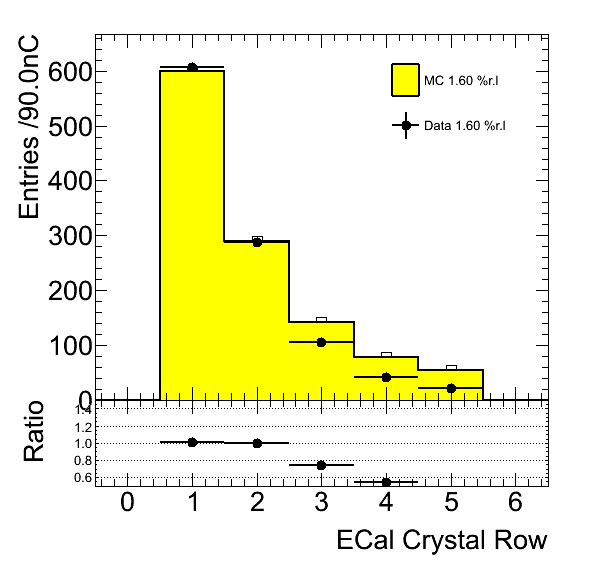
\includegraphics[ scale=0.25]{test2012/angular_measurement/pictures/dataMC_1351_Hit_Y_top_norm_bkgsub.png}
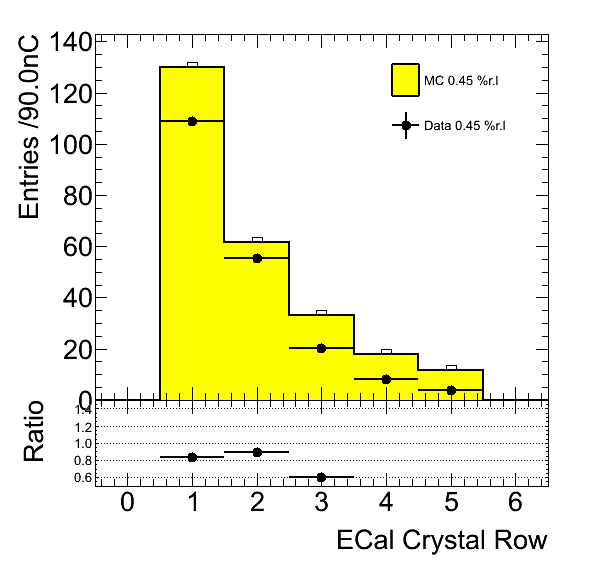
\includegraphics[ scale=0.25]{test2012/angular_measurement/pictures/dataMC_1354_Hit_Y_top_norm_bkgsub.png}
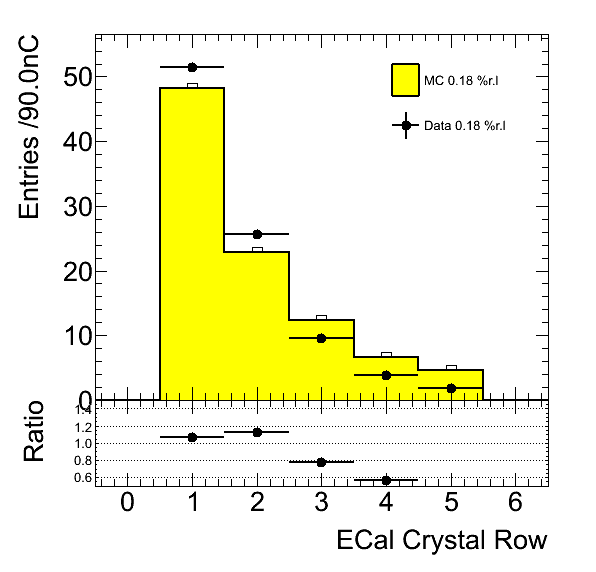
\includegraphics[ scale=0.25]{test2012/angular_measurement/pictures/dataMC_1353_Hit_Y_top_norm_bkgsub.png}
\caption{\small{Comparison between the observed and predicted angular 
distribution using EGS5 for converter thickness of 1.6\% (left), 0.45\% (middle) and 0.18\% 
(right).  Only statistical uncertainties are included. }}
\label{fig:ang_distr_dataMC}
\end{figure*}
The total rate measurements are in Fig.~\ref{fig:rate_vs_thickness} and summarized in 
Tab.~\ref{tab:ang_distr_dataMC}.
\begin{figure*}[t]
%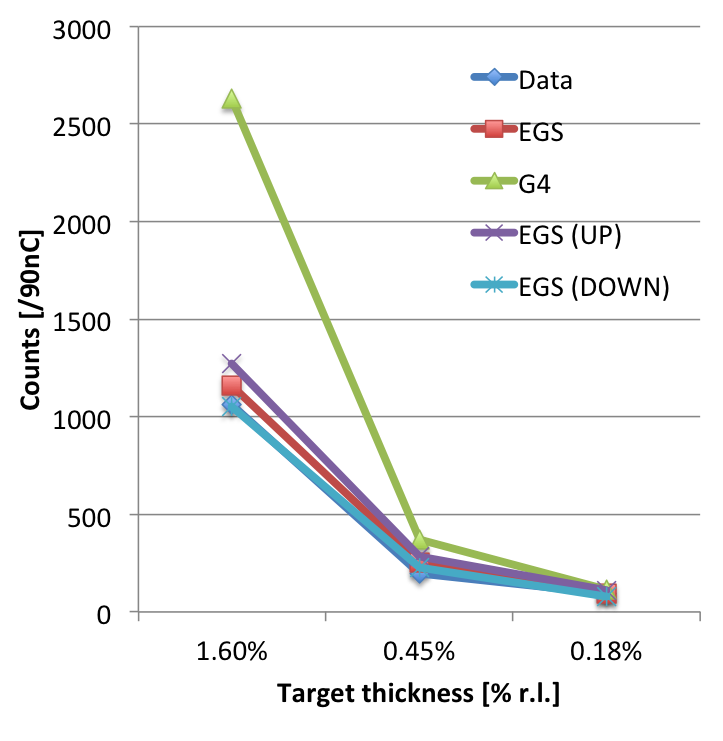
\includegraphics[ scale=0.65]{test2012/angular_measurement/pictures/rate_vs_thickness_dataMC.png}
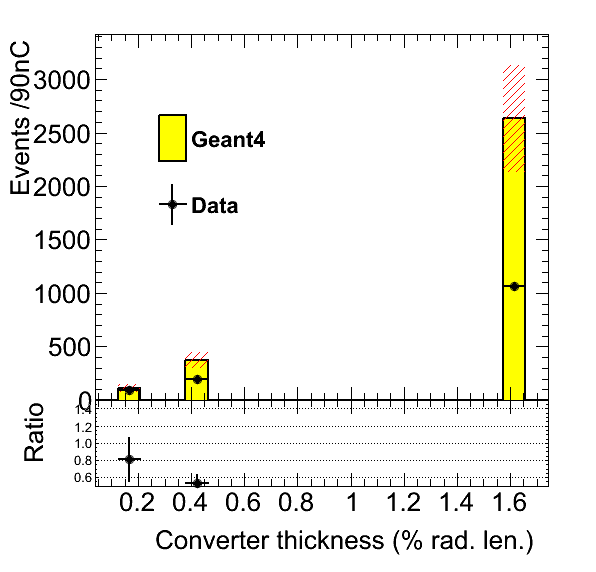
\includegraphics[ scale=0.3]{test2012/angular_measurement/pictures/dataMC_geant4.png}
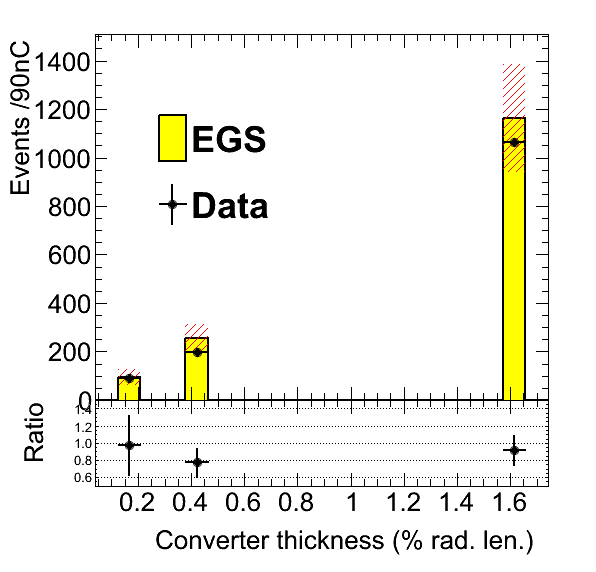
\includegraphics[ scale=0.3]{test2012/angular_measurement/pictures/dataMC_egs.png}
\caption{\small{The measured rate as a function of converter thickness comparing GEANT4 (left) and EGS5 (right)}.} 
\label{fig:rate_vs_thickness}
\end{figure*}
The total systematic uncertainty was estimated to be between 10-18\% depending on the run including:  
a 5\% uncertainty on the integrated current normalization, 
alignment of the ECal, 
uncertainty from the background normalization, 
and limited Monte Carlo statistics.  
%The uncertainty from the initial gain calibration of the 
%ECal described in Sec.{\color{red} X} was estimated to be less than {\color{red} Y\%, need to check this %calibration systematic.}.
\begin{table}
\begin{tabular}{|l|c|c|c|}
\hline
Converter (\% r.l.) & 1.60 & 0.45 &	0.18 \\
\hline
EGS5 &	1162 $\pm$ 112 &	255 $\pm$ 28 &	94 $\pm$ 17	\\
\hline
GEANT4 & 2633 $\pm$ 250 & 	371 $\pm$ 38 &	114 $\pm$ 18 \\
\hline
Observed 	& 1064 $\pm$ 2 & 196 $\pm$ 1 &	92 $\pm$ 1 \\						
%Beam gap	58	13	5	132	19	6
%	EGS			G4		
%converter thickness	1.60%	0.45%	0.18%	1.60%	0.45%	0.18%
%Data [/90nC]	1064	196	92	1064	196	92
%Pred. [/90nC]	1162	255	94	2633	371	114
%Total uncertainty	112	28	17	250	38	18
%Stat	2	1	1	2	1	1
%						
%Stat MC	11	3	1	16	3	1
%Bkg norm.	14	14	14	14	14	14
%Current norm.	94	21	8	212	30	9
%Beam gap	58	13	5	132	19	6
\hline
\end{tabular}
\caption{ {\small Observed and predicted number of events for 1~s of beam at 90~nA for three different converter 
thicknesses. The uncertainty on the prediction includes systematic uncertainties. }}
\label{tab:ang_distr_dataMC}
\end{table}

In summary, the accurate modeling of the multiple coulomb scattering is a key aspect to estimate occupancies and trigger rates for HPS. EGS5 predicts the correct angular distribution across all converter thicknesses while GEANT4 overestimates the rates; with the disagreement increasing  with larger converter thickness. This preliminary result verifies our modeling of the multiple coulomb scattering using EGS5 for HPS.
%Since EGS5 was used to generate the pair 
%angle distribution for both simulation described in the result it's interesting to see that the 
%ratio of data to the prediction varied from 0.91 (0.40), 0.77 (0.53) and 0.98 (0.81) for {\sc EGS} 
%(GEANT4) at 1.6\%, 0.45\% and 0.18\% converter thickness, respectively. If the pair angle 
%distribution were responsible for the difference between GEANT4  and EGS5 that would show up as a large shift in this ratio since the multiple coulomb scattering contribution varies. 
%There are more work needed to go from this preliminary result to a real 
%measurement. However, this preliminary result further strengthens our confidence that 
%EGS5 is able to properly describe the large angle multiple coulomb scattering events in the converter 
%which is important to estimate our occupancy and trigger rates for HPS (see Sec.~\ref{sec:performance}).
